\documentclass[10pt,a4paper]{article}

\usepackage[a4paper,top=1.8cm,bottom=1.8cm,left=2.0cm,right=2.0cm]{geometry}
\usepackage{amsmath,amssymb}
\usepackage{graphicx}
\usepackage{booktabs}
\usepackage{xcolor}
\usepackage{listings}
\usepackage{caption}
\usepackage[colorlinks=true,allcolors=blue]{hyperref}

\captionsetup{font=small,labelfont=bf}

% --- Python listing style ---
\definecolor{kw}{rgb}{0.13,0.13,0.6}
\definecolor{str}{rgb}{0.6,0.13,0.13}
\definecolor{cmt}{rgb}{0.35,0.45,0.35}
\lstdefinestyle{py}{
  language=Python,
  basicstyle=\ttfamily\scriptsize,
  keywordstyle=\color{kw}\bfseries,
  stringstyle=\color{str},
  commentstyle=\color{cmt}\itshape,
  showstringspaces=false,
  breaklines=true,
  columns=fullflexible,
  keepspaces=true,
  frame=single,
  framesep=4pt,
  rulecolor=\color{gray!40},
  aboveskip=4pt,belowskip=4pt,
}
\lstset{style=py}

\setlength{\parskip}{2pt}
\setlength{\parindent}{0pt}

\title{\vspace{-1.2cm}\textbf{Problem 1: Denoising the Egyptian Goose with PCA and NMF}}
\author{MATH70102 Unsupervised Learning --- Coursework 1}
\date{}

\begin{document}
\maketitle
\vspace{-0.9cm}

\section{Problem and approach}

We are given a clean and a noisy $512\times512$ greyscale image of an Egyptian goose, as pixel matrices $X_{\text{clean}}$ and $X_{\text{noisy}}$. For a selection of integers $q$ covering $1,\dots,512$ we reconstruct the noisy image in two ways and measure how close each reconstruction is to the clean image in \emph{Euclidean (Frobenius) distance}
\[
  d(A,B)=\sqrt{\textstyle\sum_{i,j}(A_{ij}-B_{ij})^2}.
\]
\textbf{PCA} (Week~2): treating the $512$ rows as samples in $\mathbb{R}^{512}$, we keep the first $q$ principal components and reconstruct. \textbf{NMF} (Week~3): we factorise $X_{\text{noisy}}\approx WH$ with $W\in\mathbb{R}^{512\times q}_{\ge 0}$, $H\in\mathbb{R}^{q\times 512}_{\ge 0}$ and reconstruct via $WH$. Writing $d_0=d(X_{\text{clean}},X_{\text{noisy}})$ for the baseline, a method \emph{denoises} if some $q$ gives $d(X_{\text{clean}},\hat X_q)<d_0$.

We load the data and define the distance. The noisy image is already strictly positive, so it is directly admissible to NMF without the $+1.01$ shift used in the Week~3 digit example (whose data lived in $[-1,1]$ with zeros).

\begin{lstlisting}
import matplotlib.pyplot as plt
import numpy as np
import numpy.typing as npt
from sklearn.decomposition import PCA

X_clean = np.loadtxt("egyptian_goose_clean.csv", delimiter=",")
X_noisy = np.loadtxt("egyptian_goose_noisy.csv", delimiter=",")

def euclid(A, B):                       # Euclidean / Frobenius distance
    return np.sqrt(np.sum((A - B) ** 2))

baseline = euclid(X_clean, X_noisy)     # d_0 = 29.5459
\end{lstlisting}

\section{Choosing the grid of \texorpdfstring{$q$}{q} via a scree plot}

We let the data guide the grid using a scree plot of the noisy image's principal components --- the Week~2 tool for deciding how many components to retain. The variance is heavily front-loaded (PC1 alone $\approx27\%$, PC2 $\approx14\%$; $80\%$ is reached at $q=42$, $95\%$ at $q=188$), so we sample densely at low $q$, refine over the mid-band where most variance is captured, and keep a coarse tail to $q=512$ (included as a check: there the reconstruction must equal the noisy image).

\begin{lstlisting}
scree = PCA().fit(X_noisy)
evr = scree.explained_variance_ratio_
cum = np.cumsum(evr)

fig, axs = plt.subplots(1, 2, figsize=(8, 2.7))
axs[0].bar(range(1, 31), evr[:30] * 100, color="salmon")
axs[0].set_xlabel("Principal component"); axs[0].set_ylabel("Explained variance (%)")
axs[1].plot(range(1, len(cum) + 1), cum * 100, color="royalblue")
axs[1].set_xlabel("Number of components q"); axs[1].set_ylabel("Cumulative (%)")

q_grid = np.array(sorted(set(
    list(range(1, 21))
    + [25, 30, 35, 40, 45, 50, 55, 60, 65, 70, 75, 80, 90, 100]
    + [110, 125, 150, 175, 200, 225, 250, 275, 300]
    + [350, 400, 450, 500, 512])))
\end{lstlisting}

\begin{figure}[h]
  \centering
  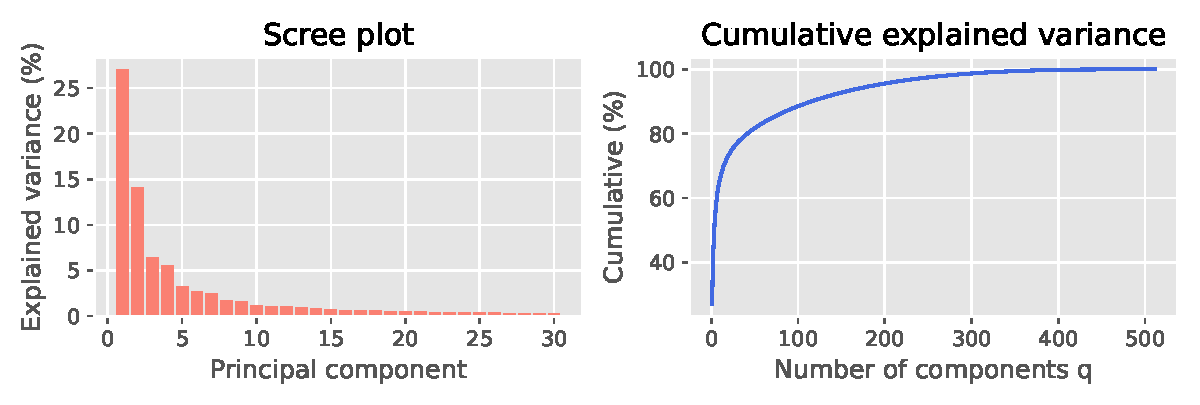
\includegraphics[width=0.86\textwidth]{fig_scree.pdf}
  \caption{Scree plot (left) and cumulative explained variance (right) of the noisy image. The steep decay justifies dense sampling at low $q$.}
\end{figure}

\section{PCA reconstruction (Week 2)}

For each $q$ we fit \texttt{PCA(n\_components=q)}, project with \texttt{fit\_transform}, and reconstruct with \texttt{inverse\_transform}. PCA re-adds the sample mean, so at $q=512$ the noisy image is recovered exactly.

\begin{lstlisting}
pca_dist = np.empty(len(q_grid)); pca_recons = {}
for i, q in enumerate(q_grid):
    pca = PCA(n_components=int(q))
    recon = pca.inverse_transform(pca.fit_transform(X_noisy))
    pca_dist[i] = euclid(X_clean, recon)
    pca_recons[int(q)] = recon

best_pca_idx = int(np.argmin(pca_dist)); best_pca_q = int(q_grid[best_pca_idx])
# PCA: best q = 80 -> d = 24.9536;  d at q=512 = 29.5459 (= baseline)
\end{lstlisting}

\section{NMF reconstruction (Week 3)}

We use the \texttt{NMF\_numpy} class from the Week~3 reference \emph{verbatim}. It maximises the quasi-likelihood $L(W,H)=\sum X\odot\log(WH)-WH$ by multiplicative updates; the reconstruction is stored in \texttt{.WH}.

\begin{lstlisting}
class NMF_numpy:
    def train(self, X: npt.NDArray[np.number], q: int, n_iter: int = 100) -> None:
        d, n = X.shape
        self.W = np.random.uniform(low=0, high=1, size=(d, q)).astype(X.dtype)
        self.H = np.random.uniform(low=0, high=1 / q, size=(q, n)).astype(X.dtype)
        self.WH = self.W @ self.H
        self.logL = np.empty(n_iter, dtype=X.dtype)
        self.dist = np.empty(n_iter, dtype=X.dtype)
        for a in range(n_iter):
            self.W *= ((X / self.WH) @ self.H.T) / self.H.sum(axis=1)[None, :]
            self.WH = self.W @ self.H
            self.H *= (self.W.T @ (X / self.WH)) / self.W.sum(axis=0)[:, None]
            self.WH = self.W @ self.H
            self.logL[a] = np.sum(X * np.log(self.WH) - self.WH)
            self.dist[a] = np.sum((X - self.WH) ** 2)
\end{lstlisting}

A convergence check at $q=20$ (Figure~\ref{fig:conv}) shows the objective flattens well before 500 iterations, so we use \texttt{n\_iter\,=\,400} in the sweep, with the random $W,H$ initialisation seeded for reproducibility.

\begin{lstlisting}
np.random.seed(0)
check = NMF_numpy(); check.train(X_noisy, q=20, n_iter=500)
fig, axs = plt.subplots(1, 2, figsize=(8, 2.4))
axs[0].plot(range(1, 501), check.logL, color="red");  axs[0].set_ylabel(r"$L(W,H)$")
axs[1].plot(range(1, 501), check.dist, color="blue"); axs[1].set_ylabel(r"$\|X-WH\|^2$")

np.random.seed(0)
nmf_dist = np.empty(len(q_grid)); nmf_recons = {}
for i, q in enumerate(q_grid):
    nmf = NMF_numpy(); nmf.train(X_noisy, int(q), n_iter=400)
    nmf_dist[i] = euclid(X_clean, nmf.WH)
    nmf_recons[int(q)] = nmf.WH

best_nmf_idx = int(np.argmin(nmf_dist)); best_nmf_q = int(q_grid[best_nmf_idx])
# NMF: best q = 275 -> d = 25.2179
\end{lstlisting}

\begin{figure}[h]
  \centering
  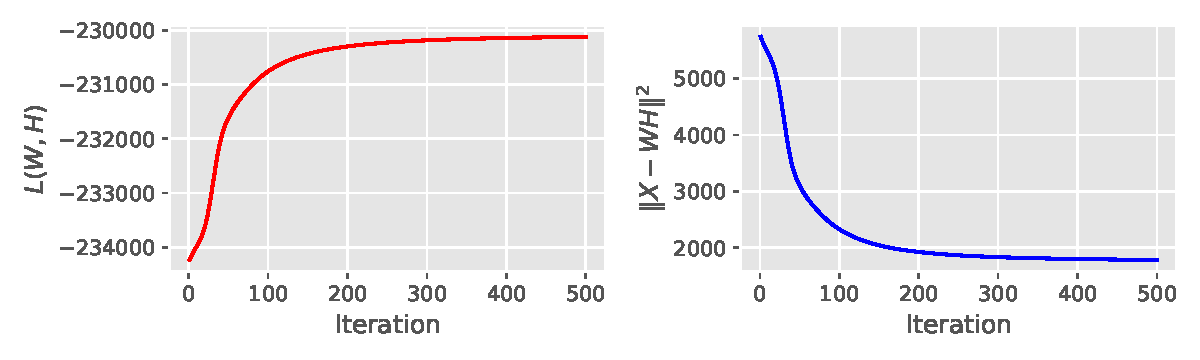
\includegraphics[width=0.72\textwidth]{fig_conv.pdf}
  \caption{NMF convergence at $q=20$: quasi-likelihood $L(W,H)$ (left) and reconstruction error $\|X-WH\|^2$ (right) against iteration. Both have plateaued by $\sim$200 iterations.}
  \label{fig:conv}
\end{figure}

\section{Results}

\begin{lstlisting}
plt.plot(q_grid, pca_dist, "-o", label="PCA")
plt.plot(q_grid, nmf_dist, "-s", label="NMF")
plt.axhline(baseline, linestyle="--", label="Baseline = %.2f" % baseline)
plt.xlabel("q"); plt.ylabel("distance to clean image"); plt.legend()
\end{lstlisting}

\begin{table}[h]
  \centering\small
  \begin{tabular}{lccccc}
    \toprule
     & best $q$ & $d(X_{\text{clean}},\hat X_q)$ & improvement vs.\ $d_0$ & cum.\ variance at $q$ & denoises? \\
    \midrule
    Baseline (noisy) & --- & $29.55$ & --- & --- & --- \\
    PCA & $80$  & $24.95$ & $4.59$ & $86\%$ & \textbf{yes} \\
    NMF & $275$ & $25.22$ & $4.33$ & $98\%$ & \textbf{yes} \\
    \bottomrule
  \end{tabular}
  \caption{Best reconstructions. PCA beats the baseline for all $q\in[25,500]$; NMF for all $q\in[35,512]$.}
\end{table}

\begin{figure}[ht!]
  \centering
  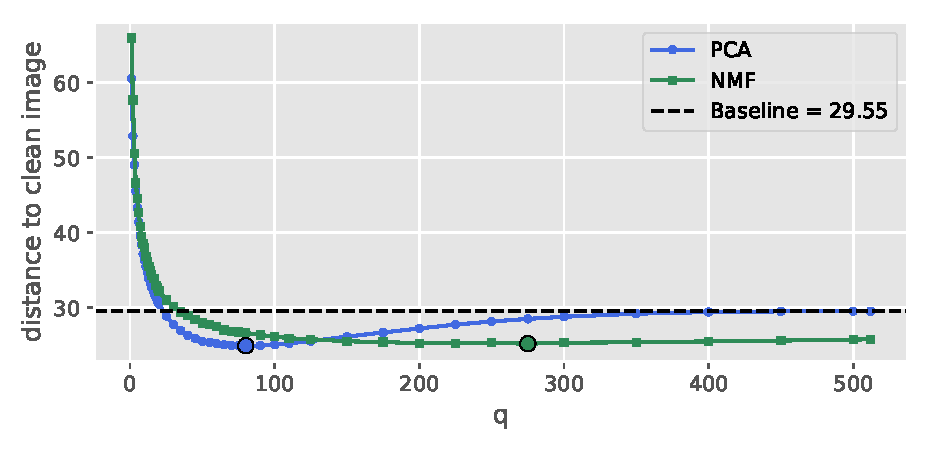
\includegraphics[width=0.90\textwidth]{fig_curve.pdf}\\[2pt]
  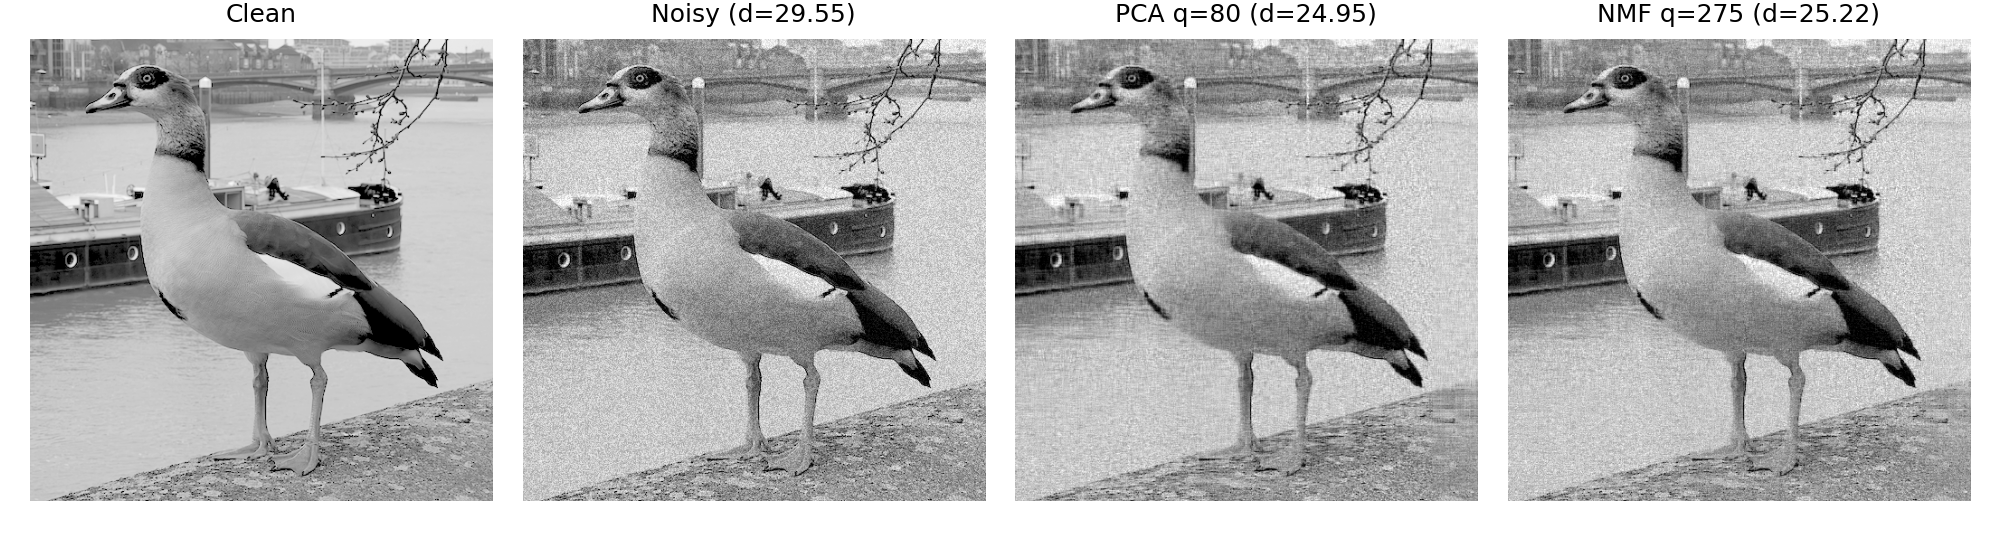
\includegraphics[width=0.99\textwidth]{fig_compare.png}
  \caption{Top: distance to the clean image versus $q$; both curves dip well below the baseline (dashed) and the marked points are the optima. Bottom: clean, noisy, and best-$q$ PCA/NMF reconstructions (displayed on the clean image's intensity range).}
\end{figure}

\vspace{-6pt}
\section{Conclusion}
\vspace{-2pt}

\textbf{Yes --- both PCA and NMF denoise the image.} For each method there is a wide band of $q$ giving a reconstruction strictly closer to the clean image than the noisy image is: the distance falls from $d_0=29.55$ to $24.95$ (PCA, $q\approx80$) and $25.22$ (NMF, $q\approx275$). The distance-versus-$q$ curve is \textbf{U-shaped}. Noise spreads its energy across all $512$ directions, whereas the image's structure is concentrated in the leading components (scree plot: PC1 $\approx27\%$). For small $q$ the reconstruction under-fits and discards genuine structure; at an intermediate $q$ it keeps the signal while rejecting the many noise-dominated high-index components --- the denoising optimum; and as $q\to512$ it recovers the noisy image ever more faithfully, so the distance climbs back to $d_0$ (for PCA this is exact, verified at $q=512$). PCA reaches its optimum earlier and slightly lower than NMF, consistent with its components being the variance-optimal directions, so it concentrates the signal into fewer of them. The improvement is real but moderate ($\approx15\%$): broadband noise can only be partly removed by a low-rank truncation, since only the portion of the noise lying in the discarded components is rejected.

\end{document}
